\begin{tikzpicture}
  \tikzset{et/.style={above,font=\footnotesize\vphantom{Ag}}}
  % 
  \node[inner sep=0pt, anchor=south west] (image) at (0,0){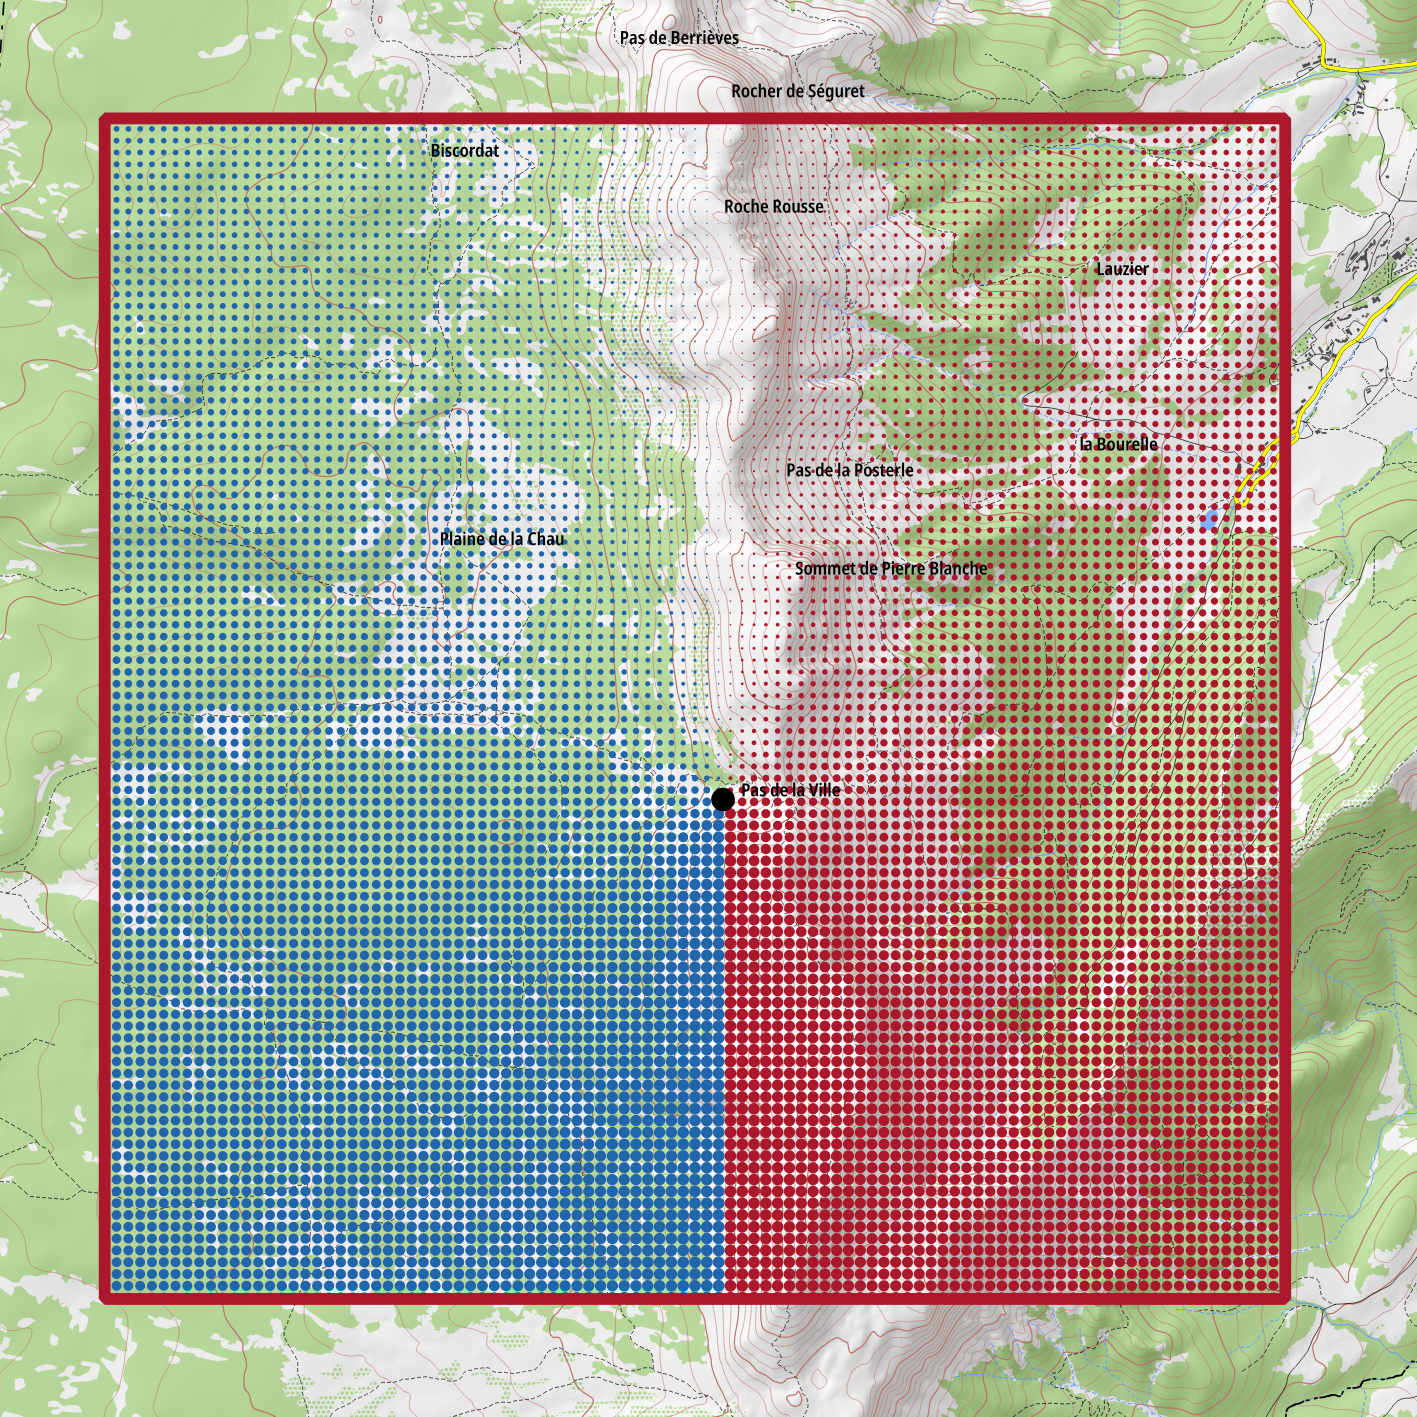
\includegraphics{./figures/EcartNord_PasVille.png}};
  % 
  \begin{scope}
    \node (P2) at ([yshift=-.5cm]image.south east) {};
    \node (P1) at ([yshift=-.5cm]image.south west) {};
    % 
    \node (rect) [anchor=north west, minimum width=1cm,minimum
    height=.25cm] at ([yshift=-.25cm]P1) {}; \path[draw=RdBu-9-1, line
    width=1mm](rect.west) --([xshift=-1ex]rect.south) -- ([xshift=1ex]rect.north)
    -- (rect.east);
    % 
    \node[anchor=west, font=\tiny\vphantom{Ag}, text width = 4cm] at
    ([xshift=1ex]rect.east) {Limite de la \ac{zir}};
    %
    \node[anchor=west, font=\footnotesize\vphantom{Ag}, text width=8cm] at
    (P1 |- 0cm,-1.85cm) {Écart angulaire à la demi-droite passant par
      le \emph{Pas de la Ville} et orientée au nord :};
    %
    \begin{scope}
      \foreach \x [evaluate=\xshift using 1+\x/10, evaluate=\rad using (\x * -.0008) + .05] in {0,...,50}
      {
        \draw[fill=RdBu-9-9,draw=none, below] ([xshift=\xshift cm, yshift=-2.5cm]P1) circle [radius=\rad cm];
      }
      \foreach \x [evaluate=\xshift using 6+\x/10, evaluate=\rad using (\x * .0008) + .01] in {0,...,50}
      {
        \draw[fill=RdBu-9-1,draw=none, below] ([xshift=\xshift cm, yshift=-2.5cm]P1) circle [radius=\rad cm];
      }
      % 
      \path(1,-3) --++ (10,0)
      node[et,pos=0] {\SI{-180}{\degre}}
      node[et,pos=.5] {\SI{0}{\degre}}
      node[et,pos=1] {\SI{180}{\degre}};
    \end{scope}

    % Échelle
    \draw[-] (P2 |- -1cm,-1cm) --++ (-1,0) node[et,pos=.5] {\SI{500}{\meter}};
    % Légende détaillée
    \path (P1) -- (P2) node[pos=.5, yshift=-3cm] {\tiny Pour la légende détaillée du fond topographique voir \autoref{anx:topo_leg}. Sources: BD TOPO 2018, BD ALTI 2018.}; 
  \end{scope}
\end{tikzpicture}